\begin{anexosenv}

\partanexos

\chapter{Telas da Aplicação}
\label{chap:telas}

\chapter{Coleta de Métricas}
\label{chap:metricas}

A figura \ref{img:rubocop} mostra o resultado da análise feita pelo rubocop. O arquivo de configuração utilizado para a análise pode ser encontrado aqui.

\begin{figure}[H]
    \centering
    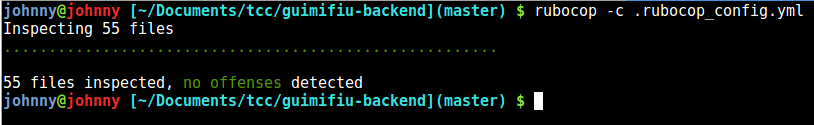
\includegraphics[scale=0.5]{figuras/rubocop.png}
    \caption[Relatório de análise estática do Rubocop]{Relatório de análise estática do Rubocop. Fonte: autores}
    \label{img:rubocop}
\end{figure}

A figura \ref{img:codeclimate} mostra o resultado das análises realizado pelo CodeClimate. 

\begin{figure}[H]
    \centering
    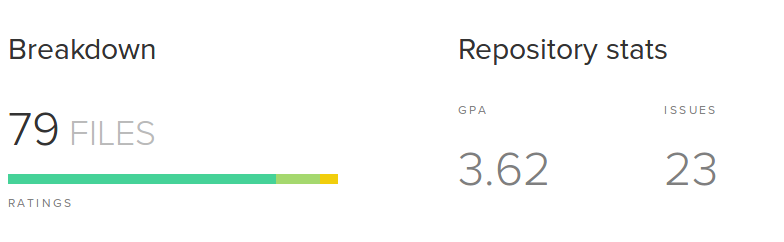
\includegraphics[scale=0.5]{figuras/codeclimate.png}
    \caption[Relatório de análise estática do CodeClimate]{Relatório de análise estática do CodeClimate. Fonte: autores}
    \label{img:codeclimate}
\end{figure}

Seis das sete \textit{issues} encontradas foram por motivo do CodeClimate utilizar um parser com uma versão menor do que a versão do Ruby utilizada pela equipe, enquanto o último foi uma duplicação de código que será tratada durante a segunda parte do trabalho.

\end{anexosenv}

